\documentclass[twoside]{article}
\setlength{\oddsidemargin}{0.25 in}
\setlength{\evensidemargin}{-0.25 in}
\setlength{\topmargin}{-0.6 in}
\setlength{\textwidth}{6.5 in}
\setlength{\textheight}{8.5 in}
\setlength{\headsep}{0.75 in}
\setlength{\parindent}{0 in}
\setlength{\parskip}{0.1 in}

\usepackage{graphicx}
\usepackage{url}

%
% The following commands sets up the lecnum (lecture number)
% counter and make various numbering schemes work relative
% to the lecture number.
%
\newcounter{lecnum}
\renewcommand{\thepage}{\thelecnum-\arabic{page}}
\renewcommand{\thesection}{\thelecnum.\arabic{section}}
\renewcommand{\theequation}{\thelecnum.\arabic{equation}}
\renewcommand{\thefigure}{\thelecnum.\arabic{figure}}
\renewcommand{\thetable}{\thelecnum.\arabic{table}}
\newcommand{\dnl}{\mbox{}\par}

%
% The following macro is used to generate the header.
%
\newcommand{\lecture}[4]{
  \pagestyle{myheadings}
  \thispagestyle{plain}
  \newpage
  \setcounter{lecnum}{#1}
  \setcounter{page}{1}
  \noindent
  \begin{center}
  \framebox{
     \vbox{\vspace{2mm}
   \hbox to 6.28in { {\bf COMPSCI~590S~~~Systems for Data Science
                       \hfill Fall 2016} }
      \vspace{4mm}
      \hbox to 6.28in { {\Large \hfill Lecture #1: #2  \hfill} }
      \vspace{2mm}
      \hbox to 6.28in { {\it Lecturer: #3 \hfill Scribe(s): #4} }
     \vspace{2mm}}
  }
  \end{center}
  \markboth{Lecture {#1}: #2}{Lecture {#1}: #2}
  \vspace*{4mm}
}

%
% Convention for citations is authors' initials followed by the year.
% For example, to cite a paper by Leighton and Maggs you would type
% \cite{LM89}, and to cite a paper by Strassen you would type \cite{S69}.
% (To avoid bibliography problems, for now we redefine the \cite command.)
%
\renewcommand{\cite}[1]{[#1]}

% \input{epsf}

%Use this command for a figure; it puts a figure in wherever you want it.
%usage: \fig{NUMBER}{FIGURE-SIZE}{CAPTION}{FILENAME}
\newcommand{\fig}[4]{
           \vspace{0.2 in}
           \setlength{\epsfxsize}{#2}
           \centerline{\epsfbox{#4}}
           \begin{center}
           Figure \thelecnum.#1:~#3
           \end{center}
   }

% Use these for theorems, lemmas, proofs, etc.
\newtheorem{theorem}{Theorem}[lecnum]
\newtheorem{lemma}[theorem]{Lemma}
\newtheorem{proposition}[theorem]{Proposition}
\newtheorem{claim}[theorem]{Claim}
\newtheorem{corollary}[theorem]{Corollary}
\newtheorem{definition}[theorem]{Definition}
\newenvironment{proof}{{\bf Proof:}}{\hfill\rule{2mm}{2mm}}

% Some useful equation alignment commands, borrowed from TeX
\makeatletter
\def\eqalign#1{\,\vcenter{\openup\jot\m@th
 \ialign{\strut\hfil$\displaystyle{##}$&$\displaystyle{{}##}$\hfil
     \crcr#1\crcr}}\,}
\def\eqalignno#1{\displ@y \tabskip\@centering
 \halign to\displaywidth{\hfil$\displaystyle{##}$\tabskip\z@skip
   &$\displaystyle{{}##}$\hfil\tabskip\@centering
   &\llap{$##$}\tabskip\z@skip\crcr
   #1\crcr}}
\def\leqalignno#1{\displ@y \tabskip\@centering
 \halign to\displaywidth{\hfil$\displaystyle{##}$\tabskip\z@skip
   &$\displaystyle{{}##}$\hfil\tabskip\@centering
   &\kern-\displaywidth\rlap{$##$}\tabskip\displaywidth\crcr
   #1\crcr}}
\makeatother

% **** IF YOU WANT TO DEFINE ADDITIONAL MACROS FOR YOURSELF, PUT THEM HERE:



% Some general latex examples and examples making use of the
% macros follow.

\begin{document}

%FILL IN THE RIGHT INFO.
%\lecture{**LECTURE-NUMBER**}{**DATE**}{**LECTURER**}{**SCRIBE**}
\lecture{5}{Sept. 20th}{Emery Berger}{Lakshmi Rajan, Timm Allman}

\section{Master-Slave Architecture}
Consider a distributed system that uses 1000 computers for performing tasks.
If the chance of any one computer failing during a given computation is 1/1000 then the probability that all the systems succeed is (1 - 1/1000)\textasciicircum1000 or about 0. This means that the probability of at least one failure is 1 - (1 - 1/1000)\textasciicircum1000 or about 100\%.

A master-slave architecture is common solution to this problem. It deals with failure by having a leader (the master) and some number of workers (the slaves). The leader divides tasks and assigns them to the workers. If the workers are slow to finish their tasks, or fail entirely, the leader reassigns those tasks to other workers so that all the work will get done (fault tolerance).
The only single point of failure is if the leader: if any of the workers die the leader will take care of it, if the leader dies there is noone to take over.

While beyond the scope of the class there are ways to “elect” a new leader. If interested look up:
  Byzantine faults/fault tolerance - Model of how failures happen and how to deal with them.
  Leslie Lamport - Computer scientist who wrote a bunch about this.
  PAXOS/RAFT - two different leader election algorithms.

\section{MapReduce}
The map-reduce paradigm has been around since Lisp. It consists of two operations: {\tt map(f, list) -$>$ list} and {\tt reduce(g, list(value)) -$>$ value} with f and g being functions. f is a unary operator that can be run in parallel on all elements of the list (it only deals with one element at a time and should be idempotent) and g is a binary operator that is (almost always) associative and commutative so the order it is applied to the list doesn’t matter.

MapReduce (MR) frameworks are more recent. The user gives the MR framework two functions: {\tt Map(key, value) -$>$ (key’, value’)} and {\tt Reduce(key’, list(value’))}. Map is run once for each item in a set and Reduce is run once for each unique key’ that Map emits.

MR uses a master-slave architecture to parallelize map and reduce over many machines. Many map and reduce tasks are runs in parallel across many systems. Because Map is idempotent (no side-effects) and stores its output into a private file it is easy for the leader to kill and reschedule map tasks without any side-effects. Similarly since Reduce is run only once per unique key’ any such task can also be easily killed and rescheduled.

Reduce is always preceded by sort operation. This is done for the following reasons:
\begin{itemize}
	\item Sort ensures that all the runs produce the same output.
	\item Results are deterministic. Hence, if an entire job is executed on one machine, or divided into tasks and executed on multiple machines, the results would be the same. This enables developers to debug and test the code locally.
\end{itemize}

Applications of MapReduce include grep, reversible web-link graph, and inverted index.

Example:
Inverted Index

{\tt Map(Url, contents) -$>$ list(word:url)}\\*
{\tt Reduce(word, list(URLs)) -$>$ list(word:urls)}\\*

Map(A, "the sandwich is delicious") -$>$ the:A; sandwich:A; is:A; delicious:A\\*
Map(B, "the pizza is delicious") -$>$ the:B; pizza:B; is:B; delicious:B\\*
Map(C, "the beer is great") -$>$ the:C; beer:C; is:C; great:C\\*

Reduce(the, list(A, B, C)) -$>$ "the":"A,B,C"\\*
Reduce(sandwich, list(A)) -$>$ "sandwich":"A"\\*
Reduce(is, list(A,B,C)) -$>$ "is":"A,B,C"\\*
Reduce(delicious, list(A,B)) -$>$ "delicious":"A,B"\\*
Reduce(pizza, list(A)) -$>$ "pizza":"A"\\*
Reduce(beer, list(C)) -$>$ "beer":"C"\\*
Reduce(great, list(C)) -$>$ "great":"C"\\*

\begin{figure}[ht!]
\centering
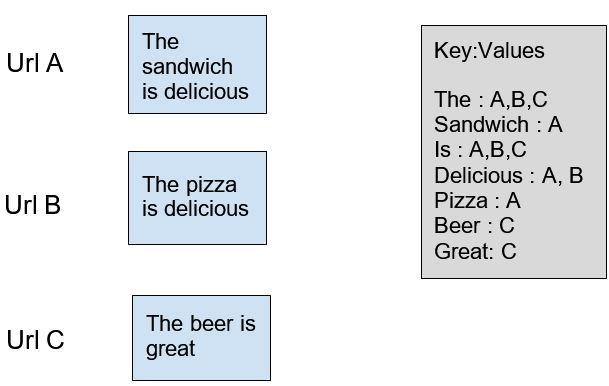
\includegraphics[width=90mm]{mapreduce_example.jpg}
\caption{Example illustrated \label{overflow}}
\end{figure}

\end{document}
